\documentclass[a4paper, 11pt]{article}
\usepackage[utf8]{inputenc}
\usepackage[T1]{fontenc} % for proper encoding hypen, dotted characterss
\usepackage{kotex} % To use Korean
\usepackage{amsmath, amsthm, amsfonts}
\usepackage{graphicx} % insert pictures.
\usepackage{tikz}
\usetikzlibrary{positioning} % To get more advances positioning options
\usetikzlibrary{arrows} % To get more arrow heads
% \usetikzlibrary{uccuuuuuuu}


\newtheorem{theorem}{Theorem}[section] % {이름}{표시}[section기반 넘버링]
\newtheorem{corollary}{Corollary}[theorem] % {이름}{표시}[theorem기반 넘버링]

\newcommand{\R}{\mathbb{R}}
\newcommand{\cv}[2]{\begin{bmatrix}
    #1 \\
    #2 \\
    \end{bmatrix}}

\title{networks}
\author{wYe}
\begin{document}

    \maketitle

    \section*{Introduction}
    Here are many examples superposition.
    $e^{\pi}+ 1 = 0$

    \begin{enumerate} % itemize
    \item 
    But we can also do
    $$
    e = \lim_{n \to \infty }\left(1+\frac{1}{n}\right)^n = \lim_{n \to \infty } \frac{n}{\sqrt[n]{n!}}
    $$

    \item We can do another.

    $$
    e = \sum_{n=0}^{\infty} \frac{1}{n!}
    $$

    \item     We can do another.

    $$
    e = 2 + \frac{1}{1+\frac{1}{2+\frac{1}{3+\frac{1}{4 + \frac{1}{5 + \ddots}}}}}
    $$
    \end{enumerate}

\section{More Formulas}
$$ \int_a^b f(x) dx $$

% amsmath
\[ \iiiint f(x, y, z) dxdydz \]

$$\vec{v}=<v_1, v_2, v_3> $$

$$ \vec{v} \cdot \vec{w} $$

$$\begin{bmatrix}
    1 & 2 & 3 \\
    4 & 5 & 6 \\
\end{bmatrix}$$

\includegraphics[scale=0.5]{mars}

\section{lectuer2 styling}

\textbf{Bold Font},
\textit{Italic Font}.
\underline{Underlined Text}

\begin{equation}
    \label{Force}
    F = ma 
    = m\frac{dv}{dt}
\end{equation}

\begin{align}
    \label{NewtonLaw}
    \frac{\partial P}{\partial t} &= 0 \\
    F_1 + F_2 &= 0 \\
\end{align}
Equation \ref{Force} was really cool!

\begin{equation}
    \begin{split}
    \frac{\partial P}{\partial t} &= 0 \\
    F_1 + F_2 &= 0 \\   
    \end{split}
\end{equation}

\begin{multline}
    x = 1 + 1 + 1 + 1 + 1 + 1 + 1 + 1 + 1 + 1\\
     + 1 + 1 + 1 + 1 + 1 + 1 
\end{multline}

\begin{table}
    \caption{a nifty table!}

    \label{niftytable}
    \begin{center}
\begin{tabular}{|c|c|}
    \hline
    1 & 2 \\ \hline
    3 & 4 \\ \hline
\end{tabular}
    \end{center}
\end{table}

I like table \ref{niftytable}.

\begin{figure}
    \centering
    \includegraphics[width=\textwidth]{mars}
    \caption{caption}
    \label{mars}
\end{figure}

I like this Mars figure \ref{mars}


\begin{theorem}[MyTheoremNamec] This is my first theorem.    
\end{theorem}
\begin{corollary}
    Yes, you know that.
\end{corollary}
\begin{proof}
    Here is the original real $\R$c proof.
\end{proof}

I write simply $\cv{1}{2}$

% Lecture 3 Theses



    \begin{tikzpicture}
        \draw (0, 0) -- (10, 0);
    \end{tikzpicture}
    style

    \begin{figure}
            
        \centering
        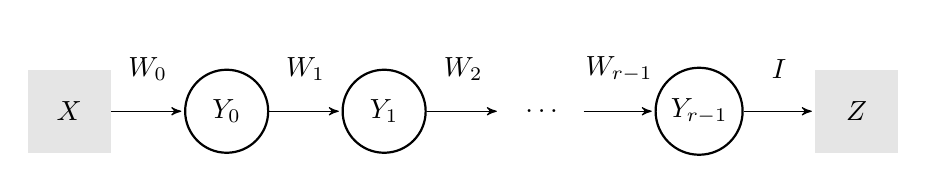
\begin{tikzpicture} [->, >=stealth',shorten >=1pt,auto,
            node distance=2.5cm,scale=1, transform shape,
            align=center,minimum size=3em]
            

            \tikzstyle{data} = [rectangle, fill=black!10]
            \tikzstyle{layer} = [circle, draw=black, thick]
            \tikzstyle{ellipsis} = []

            \node[data](input) at(0, 0) {$X$};
            \node[layer](layer_0) at(2, 0) {$Y_0$};
            \node[layer](layer_1) at(4, 0) {$Y_1$};
            \node[ellipsis](ellipsis) at(6, 0) {$\ldots$};
            \node[layer](layer_r-1) at(8, 0) {$Y_{r-1}$};
            \node[data](output) at(10, 0) {$Z$};

            \path (input) edge node {$W_0$} (layer_0)
                (layer_0) edge node {$W_1$} (layer_1)
                (layer_1) edge node {$W_2$} (ellipsis)
                (ellipsis)edge node {$W_{r-1}$} (layer_r-1)
                (layer_r-1) edge node {$I$}(output)
            ;
       \end{tikzpicture} 
       \caption{\emph{Multi-layered neural network:}
                The overall structure of a $r$-layered Neural Network looks like this.
        }
    \end{figure}



\end{document}